\documentclass[../../main.tex]{subfiles}

\graphicspath{{../../image/}{../../figure/}}

\begin{document}

\section{非参数化方法}\label{section:ch03-非参数化方法}

本章专注于使用由少量参数决定的、具有特定函数形式的概率分布，这些参数的值可从数据集中确定。这称为参数化（parametric）的密度估计方法。这种方法的一个关键局限是，所选择的密度模型可能不适合数据分布，这可能导致预测性能不佳。例如，如果生成数据的过程是多峰的，那么 Gauss 分布永远无法捕捉到分布这个角度的特征，因为 Gauss 分布必然是单峰的。本节将考虑一些非参数化（nonparametric）的密度估计方法，这些方法对分布的形式几乎不作任何假设。

\subsection{直方图}\label{subsection:ch03-直方图}

首先讨论密度估计的直方图方法。我们在前面关于边缘分布与条件分布（见\cref{figure:ch03-边缘与条件}）以及中心极限定理（见\cref{figure:ch03-中心极限直方图}）的讨论中已经见到过这种方法。下面将更详细地探讨直方图密度模型的特性，并重点关注具有单个连续变量 $x$ 的情况。标准直方图简单将 $x$ 划分为互不相交的宽度为 $\Delta_i$ 的分箱，然后计算落在不同分箱中的观测值 $x$ 的数量 $n_i$。为了将此计数值转换为归一化的概率密度，我们可以将其简单地除以观测值总数 $N$ 和分箱宽度 $\Delta_i$ 的乘积，以获得落入每个分箱的概率值：
\begin{align}
p_i=\frac{n_i}{N\Delta_i}.
\label{align:ch03-直方图密度}
\end{align}

\begin{definition}[直方图密度估计]\label{definition:ch03-直方图}
设 $x_1,\cdots,x_N$ 为一元观测值，将实轴划分为互不相交的分箱 $B_i=[b_{i-1},b_i)$，其宽度 $\Delta_i=b_i-b_{i-1}$，并记 $n_i$ 为落入第 $i$ 个分箱的观测数。称分段常数函数
\begin{align*}
\hat{p}(x)=\frac{n_i}{N\Delta_i},\qquad x\in B_i
\end{align*}
为数据的直方图密度估计（histogram density estimate）。
\end{definition}

% SUPPLEMENT: parent=definition:ch03-直方图; kind=motivation; location=紧随其后的 remark（重构新增）
\begin{remark}（重构新增）
直方图是最古老的密度估计方法，其思想是“用频率近似概率、用体积归一化”：$\frac{n_i}{N}$ 是落入第 $i$ 个分箱的经验概率，再除以箱宽 $\Delta_i$ 就把它变成密度。这样得到的 $\hat{p}$ 在每个箱内为常数，因此是阶梯函数，天然不连续。

箱宽 $\Delta_i$ 是唯一的调节参数：$\Delta_i$ 越小，阶梯越细、越能捕捉局部结构，但每箱内的样本越少、噪声越大；$\Delta_i$ 越大，估计越平滑，但会抹平真实的多峰结构（见\cref{figure:ch03-直方图示例}）。这与多项式回归中阶数 $M$ 的选择属于同一类模型复杂度问题（\cref{section:ch01-一个教学示例}）。
\end{remark}

可以看出，$\int p(x)\,\mathrm{d}x=1$。这种方法就给出了密度 $p(x)$ 的一种模型，在每个分箱的宽度上，密度是恒定的。通常情况下，我们选择具有相同宽度的分箱，$\Delta_i=\Delta$。

\begin{proposition}[直方图密度的归一性]\label{proposition:ch03-直方图归一}
设 $\hat{p}(x)=n_i/(N\Delta_i)$ 对 $x\in B_i$，诸 $B_i$ 互不相交且覆盖全部观测所在的区间，$\sum_i n_i=N$。则 $\int\hat{p}(x)\,\mathrm{d}x=1$。
\end{proposition}
\begin{proof}
（重构新增）由定义，
\begin{align*}
\int\hat{p}(x)\,\mathrm{d}x=\sum_i\int_{B_i}\frac{n_i}{N\Delta_i}\,\mathrm{d}x=\sum_i\frac{n_i}{N\Delta_i}\cdot\Delta_i=\frac{1}{N}\sum_i n_i=1,
\end{align*}
因为每个观测恰好落入一个分箱，故 $\sum_i n_i=N$。
\end{proof}

% SUPPLEMENT: parent=proposition:ch03-直方图归一; kind=motivation; location=紧随其后的 remark（重构新增）
\begin{remark}（重构新增）
归一化成立的前提是“分箱覆盖了全部观测”，若把观测范围之外的部分也算入积分，则需要额外规定 $\hat{p}=0$，此时归一化仍然成立。这条性质说明直方图是一个合法的密度模型，而不是任意的高度堆叠。

注意归一化并不要求各箱等宽：$\Delta_i$ 可以不同，只要每箱按自己的宽度作除法即可。等宽只是常见约定，便于比较各箱高度。
\end{remark}

\cref{figure:ch03-直方图示例}展示了直方图密度估计的示例。这里的数据来自绿色曲线所对应的分布，该分布由两个 Gauss 分布混合形成。这 3 个直方图密度估计的例子对应着 3 种不同的分箱宽度 $\Delta$。我们可以看到，当 $\Delta$ 非常小时（\cref{figure:ch03-直方图示例}的顶部图），得到的密度模型非常毛糙，具有许多在生成数据集的底层分布中不存在的结构。相反，如果 $\Delta$ 太大（\cref{figure:ch03-直方图示例}的底部图），得到的密度模型将太过平滑，因此无法捕捉到绿色曲线的双峰特性。最佳结果是 $\Delta$ 取某个中间值（\cref{figure:ch03-直方图示例}的中间图）。原则上，直方图密度模型还取决于分箱边界的选择，但这相较于分箱宽度 $\Delta$ 的选择来说通常不那么重要。

\begin{figure}[htbp]
  \centering
  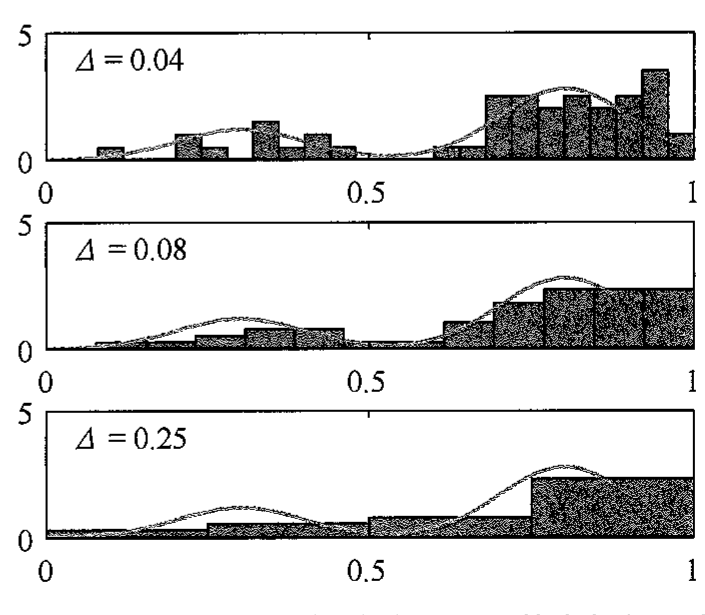
\includegraphics[width=0.60\textwidth]{ch03-fig3-13-histogram.png}
  \caption{直方图密度估计的示例，其中根据绿色曲线所示的分布生成含有 50 个数据点的数据集。这里的直方图密度估计基于\eqref{align:ch03-直方图密度}，具有相同的分箱宽度 $\Delta_i$。图中展示了不同分箱宽度的结果。}
  \label{figure:ch03-直方图示例}
\end{figure}

注意直方图方法具有一个特性（与稍后讨论的其他密度估计方法不同），即一旦直方图计算完成，数据集本身就可以丢弃，这一点在数据集很大时会十分有利。如果数据点是顺序到达的，则应用直方图方法也将比较容易。

在实践中，直方图技术可以用于快速可视化一维或二维数据，但其不适用于大多数密度估计应用。一个明显的问题是，分箱边界导致估计的密度是不连续的，而这并不是由生成数据的底层分布的任何性质引起的。直方图方法的一个主要局限是，规模会随维度变化显著改变。如果将 $D$ 维空间中的每个变量划分为 $M$ 个区间，那么分箱将有 $M^{D}$ 个。这种随 $D$ 指数级扩展的特性是维度诅咒（curse of dimensionality）的一个例子（参见\cref{subsection:ch06-维度诅咒}）。在高维空间中，为了提供有意义的局部概率密度估计，所需的数据量将是我们无法承受的。

然而，直方图方法也给密度估计带来了两条重要的经验。首先，要在特定位置估计概率密度，就应该考虑落在该位置某个局部邻域内的数据点。注意局部性的概念要求我们假设某种距离度量，而在这里我们假设的是欧氏距离。对于直方图来说，这种邻域性质是由分箱定义的，并且存在一个自然的“平滑”参数用于描述局部区域的空间大小，本例中即为分箱宽度。其次，为了获得良好的结果，平滑参数的值既不应该太大也不应该太小。这会让人联想到多项式回归中模型复杂性的选择（参见\cref{section:ch01-一个教学示例}），其中多项式的阶数 $M$ 或者正则化参数 $\lambda$ 在某些中间值上是最优的，既不太大也不太小。有了这些洞察，下面我们来讨论两种使用广泛的非参数化密度估计技术——核密度和最近邻，它们在维度变化时的扩展性比简单的直方图模型要好。

\begin{remark}（重构新增）
这一段实际上给出了非参数密度估计的“方法论总结”：任何局部方法都由两件事决定——邻域的定义方式（距离、形状、大小）与平滑参数的选取。直方图把邻域固定为分箱，因此其平滑参数就是箱宽；核密度把邻域固定为形状给定、宽度为 $h$ 的核；最近邻则让邻域大小随数据密度自适应变化。

分箱边界造成的不连续是直方图的固有问题：它不是数据本身的性质，而是人为网格的产物。改进方向有两个：用光滑核代替指示函数（消除不连续），或让邻域随位置自适应（缓解高维稀疏）。这两种改进分别对应\cref{subsection:ch03-核密度}与\cref{subsection:ch03-最近邻}。
\end{remark}

\subsection{核密度}\label{subsection:ch03-核密度}

假设观测值是从某个 $D$ 维空间（这里将其视为欧氏空间）中的某个未知概率密度 $p(\boldsymbol{x})$ 中产生的，我们希望估计 $p(\boldsymbol{x})$ 的值。根据先前关于局部性的讨论，考虑包含 $\boldsymbol{x}$ 的一个小区域 $\mathcal{R}$。与该区域相关联的概率质量为
\begin{align}
P=\int_{\mathcal{R}}p(\boldsymbol{x})\,\mathrm{d}\boldsymbol{x}.
\label{align:ch03-区域概率}
\end{align}
假设我们已经收集了一个包含 $N$ 个从 $p(\boldsymbol{x})$ 中产生的观测值的数据集。因为每个数据点在 $\mathcal{R}$ 内的概率为 $P$，所以 $\mathcal{R}$ 内的点的总数 $K$ 将服从二项分布（参见\cref{subsection:ch03-二项分布}）：
\begin{align}
\mathrm{Bin}(K\mid N,P)=\frac{N!}{K!\,(N-K)!}P^{K}(1-P)^{N-K}.
\label{align:ch03-区域二项}
\end{align}
利用\eqref{align:ch03-二项均值}可以看出，落入该区域的点的平均占比为 $\mathbb{E}[K/N]=P$。类似地，利用\eqref{align:ch03-二项方差}可以看出，此均值对应的方差为 $\mathrm{var}[K/N]=P(1-P)/N$。对于较大的 $N$，该分布在均值处将变得十分尖锐，因此
\begin{align}
K\approx NP.
\label{align:ch03-近邻计数}
\end{align}
然而，如果我们同时假设区域 $\mathcal{R}$ 足够小，以至于概率密度 $p(\boldsymbol{x})$ 在该区域内大致保持恒定，则有
\begin{align}
P\approx p(\boldsymbol{x})V,
\label{align:ch03-局部概率}
\end{align}
其中 $V$ 是区域 $\mathcal{R}$ 的体积。结合\eqref{align:ch03-近邻计数}和\eqref{align:ch03-局部概率}，可以得到密度估计的形式为
\begin{align}
p(\boldsymbol{x})=\frac{K}{NV}.
\label{align:ch03-局部密度}
\end{align}

\begin{proposition}[局部密度估计]\label{proposition:ch03-局部密度}
设区域 $\mathcal{R}$ 包含 $\boldsymbol{x}$、体积为 $V$，$N$ 个独立样本中有 $K$ 个落入 $\mathcal{R}$。若 $p$ 在 $\mathcal{R}$ 内近似为常数且 $N$ 充分大，则
\begin{align*}
p(\boldsymbol{x})\approx\frac{K}{NV}.
\end{align*}
\end{proposition}
\begin{proof}
（重构新增）把落入 $\mathcal{R}$ 视为一次“成功”概率为 $P$ 的 Bernoulli 试验，则 $K\sim\mathrm{Bin}(K\mid N,P)$，即\eqref{align:ch03-区域二项}。由\cref{proposition:ch03-二项矩}，$\mathbb{E}[K/N]=P$、$\mathrm{var}[K/N]=P(1-P)/N$。当 $N\to\infty$ 时方差趋于零，故 $K/N$ 依概率收敛到 $P$，即 $K\approx NP$（\eqref{align:ch03-近邻计数}）。

另一方面，若 $p$ 在 $\mathcal{R}$ 内近似为常数，则\eqref{align:ch03-区域概率}给出 $P=\int_{\mathcal{R}}p\,\mathrm{d}\boldsymbol{x}\approx p(\boldsymbol{x})V$（\eqref{align:ch03-局部概率}）。两式联立消去 $P$ 得 $p(\boldsymbol{x})\approx K/(NV)$，即\eqref{align:ch03-局部密度}。
\end{proof}

% SUPPLEMENT: parent=proposition:ch03-局部密度; kind=motivation; location=紧随其后的 remark（重构新增）
\begin{remark}（重构新增）
\eqref{align:ch03-局部密度}是本节所有非参数方法的共同出发点：它把“估计密度”转化为“数一数邻域里有多少点、再除以体积”。核密度与最近邻的区别只在于固定 $V$ 还是固定 $K$。

注意式\eqref{align:ch03-局部密度}的有效性依靠两个相互矛盾的假设：区域 $\mathcal{R}$ 足够小，以至于密度在该区域内近似恒定；但区域 $\mathcal{R}$ 又足够大（与该区域内密度的值相关），使得落入该区域的点的数量 $K$ 足以使二项分布变得十分尖锐。$V$ 的选取就是在这两个要求之间折中，这正是平滑参数 $h$（或 $K$）要解决的问题。此外，$N\to\infty$ 时还需 $V\to0$ 而 $NV\to\infty$，才能同时保证偏差与方差都趋于零。
\end{remark}

我们可以通过两种不同的方式利用\eqref{align:ch03-局部密度}。一种是固定 $K$ 并根据数据确定 $V$ 的值，这将引出后面讨论的 $K$ 近邻技术；另一种是固定 $V$ 并根据数据确定 $K$ 的值，从而引出核密度估计技术。可以证明，当 $N\to\infty$ 时，只要 $V$ 随着 $N$ 以合适的速率缩小，而 $K$ 随着 $N$ 以合适的速率增长，$K$ 近邻密度估计和核密度估计都会收敛到真实概率密度（Duda and Hart, 1973）。

下面详细讨论核密度估计技术。首先，对于希望确定概率密度的点 $\boldsymbol{x}$，将区域 $\mathcal{R}$ 取为以点 $\boldsymbol{x}$ 为中心的超小立方体。为了计算落入该区域的点的数量 $K$，定义如下函数：
\begin{align}
k(\boldsymbol{u})=\begin{cases}1, & \lvert u_i\rvert\leqslant1/2,\ i=1,\cdots,D,\\ 0, & \text{其他}.\end{cases}
\label{align:ch03-Parzen窗}
\end{align}

\begin{definition}[核函数与 Parzen 窗]\label{definition:ch03-核函数}
称满足 $k(\boldsymbol{u})\geqslant0$ 且 $\int k(\boldsymbol{u})\,\mathrm{d}\boldsymbol{u}=1$ 的函数 $k$ 为核函数（kernel function）。由\eqref{align:ch03-Parzen窗}给出的 $k$ 表示以原点为中心的单位立方体，又称为 Parzen 窗（Parzen window）。
\end{definition}

% SUPPLEMENT: parent=definition:ch03-核函数; kind=motivation; location=紧随其后的 remark（重构新增）
\begin{remark}（重构新增）
核函数的作用是把“点是否落在邻域内”这一硬判定换成可加权的“相似度”：Parzen 窗是 0/1 的硬判定（在立方体内为 $1$，否则为 $0$），因此它对应的密度估计仍是阶梯状的、在立方体边界上不连续；若把 $k$ 换成光滑函数（如 Gauss 核），得到的密度也就光滑了。

定义中的两个条件各有含义：非负性保证估计出的密度非负；归一化 $\int k=1$ 保证每个数据点对总概率质量的贡献恰好为 $1$，从而整体密度可归一（见\cref{proposition:ch03-核密度归一}）。注意 $k$ 不必对称，但对称核在直观上更自然。
\end{remark}

它表示以原点为中心的单位立方体。函数 $k(\boldsymbol{u})$ 是一个核函数，在这里，它又称为 Parzen 窗。根据\eqref{align:ch03-Parzen窗}，如果数据点 $\boldsymbol{x}_n$ 位于以点 $\boldsymbol{x}$ 为中心、边长为 $h$ 的立方体内，那么量 $k((\boldsymbol{x}-\boldsymbol{x}_n)/h)$ 将为 $1$，否则为 $0$。因此，位于该立方体内的数据点的总数为
\begin{align}
K=\sum_{n=1}^{N}k\left(\frac{\boldsymbol{x}-\boldsymbol{x}_n}{h}\right).
\label{align:ch03-核计数}
\end{align}
将\eqref{align:ch03-核计数}代入\eqref{align:ch03-局部密度}，可得点 $\boldsymbol{x}$ 处估计的密度为
\begin{align}
p(\boldsymbol{x})=\frac{1}{N}\sum_{n=1}^{N}\frac{1}{h^{D}}\,k\!\left(\frac{\boldsymbol{x}-\boldsymbol{x}_n}{h}\right),
\label{align:ch03-核密度估计}
\end{align}
这里使用了 $D$ 维空间中边长为 $h$ 的超小立方体的体积公式 $V=h^{D}$。利用函数 $k(\boldsymbol{u})$ 的对称性，我们可以不再将其视为以点 $\boldsymbol{x}$ 为中心的单个立方体，而是视为以 $N$ 个数据点 $\boldsymbol{x}_n$ 为中心的 $N$ 个立方体的总和，进而重新解释这个方程。

\begin{definition}[核密度估计]\label{definition:ch03-核密度}
设 $k$ 为核函数，$h>0$ 为带宽（平滑参数）。称由\eqref{align:ch03-核密度估计}定义的函数 $\hat{p}$ 为数据 $\{\boldsymbol{x}_n\}$ 的核密度估计（kernel density estimate），又称 Parzen 估计。
\end{definition}

% SUPPLEMENT: parent=definition:ch03-核密度; kind=motivation; location=紧随其后的 remark（重构新增）
\begin{remark}（重构新增）
\eqref{align:ch03-核密度估计}的两种读法都很有用：从“以 $\boldsymbol{x}$ 为中心”看，它是“数邻域内的点数再除以体积”；从“以数据点为中心”看，它是“在每个数据点上放一个核、再把 $N$ 个核平均”。后一种读法直接说明了为什么核密度估计总是光滑的（只要核光滑）、为什么它的计算量是 $O(N)$、以及为什么它天然是一个合法密度（核的非负性与归一性会被继承）。

带宽 $h$ 扮演平滑参数的角色：$h$ 太小则每个核过于尖锐，估计出现许多虚假尖峰（对噪声敏感）；$h$ 太大则核相互重叠过度，多峰结构被抹平。这一权衡与直方图的箱宽选择完全平行（\cref{figure:ch03-核密度示例}）。
\end{remark}

就目前情况来看，核密度估计[\eqref{align:ch03-核密度估计}]将遇到与直方图方法相同的一个问题，即存在人为的不连续性，此处体现在立方体的边界上。如果我们选择更平滑的核函数，则可以获得更平滑的密度模型。我们通常选择使用 Gauss 函数，导出的核密度模型为
\begin{align}
p(\boldsymbol{x})=\frac{1}{N}\sum_{n=1}^{N}\frac{1}{(2\pi h^{2})^{D/2}}\exp\left\{-\frac{\lVert\boldsymbol{x}-\boldsymbol{x}_n\rVert^{2}}{2h^{2}}\right\}.
\label{align:ch03-Gauss核密度}
\end{align}
其中 $h$ 代表所使用 Gauss 分量的标准差。因此，我们得到密度模型的方式是，首先在每个数据点上放置一个 Gauss 分布，并将整个数据集的贡献相加，然后除以 $N$ 来正确地归一化密度。在\cref{figure:ch03-核密度示例}中，核密度模型[\eqref{align:ch03-Gauss核密度}]被应用于之前展示直方图方法的数据集。正如预期的那样，我们可以看到参数 $h$ 充当了平滑参数的角色，并且 $h$ 较小时对噪声敏感，与 $h$ 较大时过度平滑之间存在权衡。同样，类似于直方图密度估计中的分箱选择或曲线拟合中所使用多项式的阶数选择，$h$ 的优化是模型复杂性的问题。

\begin{figure}[htbp]
  \centering
  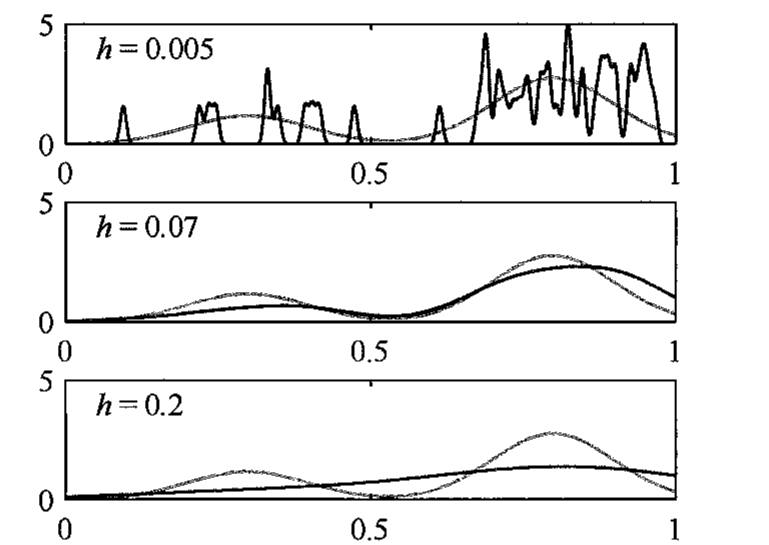
\includegraphics[width=0.60\textwidth]{ch03-fig3-14-kde.png}
  \caption{核密度模型[\eqref{align:ch03-Gauss核密度}]的图示。这里使用与前面展示直方图方法时相同的数据集。我们可以看到 $h$ 充当了平滑参数的角色，如果 $h$ 设置得太小（顶部图），则结果是噪声很大的核密度模型；而如果 $h$ 设置得太大（底部图），那么所生成数据的底层分布（绿色曲线）的双峰性质就会被淡化。通过对 $h$ 取某个中间值，可以获得最佳的核密度模型（中间图）。}
  \label{figure:ch03-核密度示例}
\end{figure}

我们可以在\eqref{align:ch03-指数族定义}中选择任何其他核函数 $k(\boldsymbol{u})$，只要满足以下两个条件即可。
\begin{align}
k(\boldsymbol{u})\geqslant0,
\label{align:ch03-核非负}
\end{align}
\begin{align}
\int k(\boldsymbol{u})\,\mathrm{d}\boldsymbol{u}=1.
\label{align:ch03-核归一}
\end{align}
这两个条件确保了得到的概率分布在任何地方都是非负的，并且积分为 $1$。由\eqref{align:ch03-核密度估计}给出的这类密度模型称为核密度估计器或 Parzen 估计器。

\begin{proposition}[核密度估计的归一性]\label{proposition:ch03-核密度归一}
设 $k$ 满足\eqref{align:ch03-核非负}与\eqref{align:ch03-核归一}，则由\eqref{align:ch03-核密度估计}定义的 $\hat{p}$ 满足 $\hat{p}(\boldsymbol{x})\geqslant0$ 与 $\int\hat{p}(\boldsymbol{x})\,\mathrm{d}\boldsymbol{x}=1$。
\end{proposition}
\begin{proof}
（重构新增）非负性：由\eqref{align:ch03-核非负}，$k((\boldsymbol{x}-\boldsymbol{x}_n)/h)\geqslant0$，故\eqref{align:ch03-核密度估计}右端是若干非负项之和，必非负。

归一性：作变量替换 $\boldsymbol{u}=(\boldsymbol{x}-\boldsymbol{x}_n)/h$，则 $\mathrm{d}\boldsymbol{x}=h^{D}\mathrm{d}\boldsymbol{u}$，于是
\begin{align*}
\int\hat{p}(\boldsymbol{x})\,\mathrm{d}\boldsymbol{x}=\frac{1}{N}\sum_{n=1}^{N}\frac{1}{h^{D}}\int k\!\left(\frac{\boldsymbol{x}-\boldsymbol{x}_n}{h}\right)\mathrm{d}\boldsymbol{x}=\frac{1}{N}\sum_{n=1}^{N}\int k(\boldsymbol{u})\,\mathrm{d}\boldsymbol{u}=\frac{1}{N}\cdot N\cdot1=1,
\end{align*}
其中用到\eqref{align:ch03-核归一}。
\end{proof}

% SUPPLEMENT: parent=proposition:ch03-核密度归一; kind=motivation; location=紧随其后的 remark（重构新增）
\begin{remark}（重构新增）
这两条结论说明“核的条件”正是“估计量是密度”的充分条件：核非负 $\Rightarrow$ 估计非负，核归一 $\Rightarrow$ 估计归一。因此，任何满足这两个条件的函数都可以拿来当核，而不必是立方体或 Gauss 函数——常见的选择还有 Epanechnikov 核、均匀核、三角核等。

注意归一化依赖于因子 $1/h^{D}$（$D$ 维体积缩放），少了它就只对 $k$ 的某个特定形状成立。这也解释了为什么带宽 $h$ 同时控制“平滑程度”与“密度的高度”。
\end{remark}

它们有一个很大的优点，就是在“训练”阶段不涉及计算，因为只需要将训练集存储起来即可。然而，这同时也是这类密度模型的一个巨大缺点，因为评估密度的计算成本会随着数据集的增大而线性增长。

\subsection{最近邻}\label{subsection:ch03-最近邻}

使用核方法进行密度估计的一个难点在于，对所有核来说控制核宽度的参数 $h$ 是固定的。在数据密度较高的区域，较大的 $h$ 值可能导致过度平滑，并且可能淡化从数据中本应提取出的结构。然而，减小 $h$ 值可能会导致在其他数据密度较低的区域产生噪声估计。因此，$h$ 的最佳选择可能取决于数据空间中的位置。这个问题可以通过使用最近邻方法进行密度估计来解决。

因此，下面我们重新回到局部密度估计的一般结果[\eqref{align:ch03-局部密度}]。我们不使用固定 $V$ 值并从数据中确定 $V$ 值的方式，而是考虑固定 $K$ 值并使用数据找到适当的 $V$ 值。为此，对于希望估计密度 $p(\boldsymbol{x})$ 的点 $\boldsymbol{x}$，考虑以点 $\boldsymbol{x}$ 为中心的小球，并允许小球的半径增长，直至恰好包含 $K$ 个数据点。然后，密度 $p(\boldsymbol{x})$ 的估计由\eqref{align:ch03-局部密度}给出，其中 $V$ 设置为小球的体积。

\begin{definition}[$K$ 近邻密度估计]\label{definition:ch03-近邻密度}
设 $K$ 为正整数，对给定的点 $\boldsymbol{x}$，记 $V(\boldsymbol{x})$ 为以 $\boldsymbol{x}$ 为中心、恰好包含 $K$ 个训练数据点的最小球的体积。称
\begin{align*}
\hat{p}(\boldsymbol{x})=\frac{K}{N\,V(\boldsymbol{x})}
\end{align*}
为 $K$ 近邻（$K$ nearest neighbor）密度估计。
\end{definition}

% SUPPLEMENT: parent=definition:ch03-近邻密度; kind=motivation; location=紧随其后的 remark（重构新增）
\begin{remark}（重构新增）
最近邻方法把“固定体积”换成“固定点数”，从而使邻域大小随数据密度自适应：在数据稠密处，只要很小的球就能凑够 $K$ 个点，因此 $V$ 小、估计更细致；在数据稀疏处，球必须张得很大，$V$ 大、估计被平滑。这正好解决了核方法“全局固定 $h$”的困难。

$K$ 扮演平滑参数的角色：$K$ 太小则对噪声敏感（$V$ 由最近的几个点决定，波动大），$K$ 太大则过度平滑（$V$ 覆盖太大区域）。注意 $\hat{p}$ 一般不是真正的密度——它在整个空间上的积分发散（\cref{exercise:ch03-38}），这是它作为“局部估计”的代价。
\end{remark}

\cref{figure:ch03-近邻密度示例}展示了在使用与\cref{figure:ch03-直方图示例}和\cref{figure:ch03-核密度示例}中相同的数据集的情况下，选择不同参数 $K$ 时的 $K$ 近邻密度估计。我们可以看到 $K$ 值决定了模型的平滑程度，而且同样存在一个既不太大也不太小的最佳 $K$ 值。注意 $K$ 近邻产生的模型并不是一个真正的密度模型，因为其在整个空间上的积分是发散的（见\cref{exercise:ch03-38}）。

\begin{figure}[htbp]
  \centering
  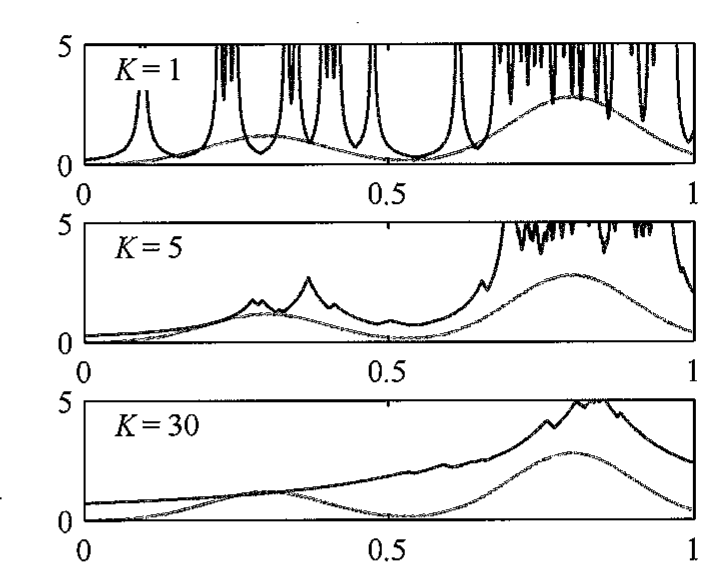
\includegraphics[width=0.55\textwidth]{ch03-fig3-15-knn-density.png}
  \caption{$K$ 近邻密度估计的图示，使用与前面展示直方图方法和核密度方法时相同的数据集。可以看到参数 $K$ 控制了模型的平滑程度，因此较小的 $K$ 值会导致噪声极大的密度模型（顶部图），而较大的 $K$ 值则会平滑掉所生成数据的真实分布（绿色曲线）的双峰性质（底部图）。}
  \label{figure:ch03-近邻密度示例}
\end{figure}

下面通过展示 $K$ 近邻技术如何扩展到分类问题来结束本章。为此，我们需要将 $K$ 近邻密度估计分别应用于每个类别，然后利用 Bayes 定理。假设数据集包含 $N_k$ 个属于类别 $C_k$ 的点，总共有 $N$ 个点，即 $\sum_k N_k=N$。如果希望对一个新点 $\boldsymbol{x}$ 进行分类，则可以在这个点的周围绘制一个恰好包含 $K$ 个点的球体，这里不考虑它们的类别。假设这个球体的体积为 $V$，并且包含来自类别 $C_k$ 的 $K_k$ 个点。\eqref{align:ch03-局部密度}提供了与每个类别相关联的密度估计值：
\begin{align}
p(\boldsymbol{x}\mid C_k)=\frac{K_k}{N_kV}.
\label{align:ch03-近邻条件密度}
\end{align}
类似地，无条件密度由下式给出：
\begin{align}
p(\boldsymbol{x})=\frac{K}{NV}.
\label{align:ch03-近邻无条件密度}
\end{align}
类别先验由下式给出：
\begin{align}
p(C_k)=\frac{N_k}{N}.
\label{align:ch03-近邻先验}
\end{align}
我们现在可以使用 Bayes 定理结合\eqref{align:ch03-近邻条件密度}至\eqref{align:ch03-近邻先验}得到类别成员的后验概率：
\begin{align}
p(C_k\mid\boldsymbol{x})=\frac{p(\boldsymbol{x}\mid C_k)p(C_k)}{p(\boldsymbol{x})}=\frac{K_k}{K}.
\label{align:ch03-近邻后验}
\end{align}

\begin{proposition}[$K$ 近邻分类的后验概率]\label{proposition:ch03-近邻分类}
设按\eqref{align:ch03-近邻条件密度}至\eqref{align:ch03-近邻先验}定义各类密度、总密度与类先验，则后验概率为 $p(C_k\mid\boldsymbol{x})=K_k/K$，其中 $K_k$ 是球体内属于类别 $C_k$ 的点数，$K=\sum_k K_k$。
\end{proposition}
\begin{proof}
（重构新增）由 Bayes 定理，
\begin{align*}
p(C_k\mid\boldsymbol{x})=\frac{p(\boldsymbol{x}\mid C_k)p(C_k)}{p(\boldsymbol{x})}=\frac{\dfrac{K_k}{N_kV}\cdot\dfrac{N_k}{N}}{\dfrac{K}{NV}}=\frac{K_k}{K},
\end{align*}
其中 $V$ 与 $N$ 在分子分母中相消，$N_k$ 也相消。
\end{proof}

% SUPPLEMENT: parent=proposition:ch03-近邻分类; kind=motivation; location=紧随其后的 remark（重构新增）
\begin{remark}（重构新增）
这个结果极其简洁：后验概率就是“球内该类点数占球内总点数的比例”。它说明 $K$ 近邻分类完全不需要显式估计密度，只需要数点数——这正是非参数方法“把估计问题化为计数问题”的典型体现。

注意推导中假设各类共享同一个球体与同一个 $V$（即同一个 $K$），否则三个式子中的 $V$ 不能相消。$K_k/K$ 的估计误差随 $K$ 增大而减小，但 $K$ 增大会使球体跨越类别边界、引入偏差，因此 $K$ 的选择仍是偏差—方差权衡。
\end{remark}

我们可以通过将测试点 $\boldsymbol{x}$ 分配给具有最大后验概率的类别来最小化错误分类的概率，这对应于 $K_k/K$ 的最大值。因此，在对一个新点进行分类时，我们首先需要识别训练集中与新点最近的 $K$ 个点，然后将新点分配给在这组点中拥有最多代表的类别。如果多个类别拥有的代表数量一致，则可以将新点随机分配给其中一个类别。$K=1$ 的特殊情况称为最近邻法则，因为测试点被简单地分配给了训练集中离新点最近的点所属的那个类别。\cref{figure:ch03-近邻分类}对这些概念进行了说明。

\begin{figure}[htbp]
  \centering
  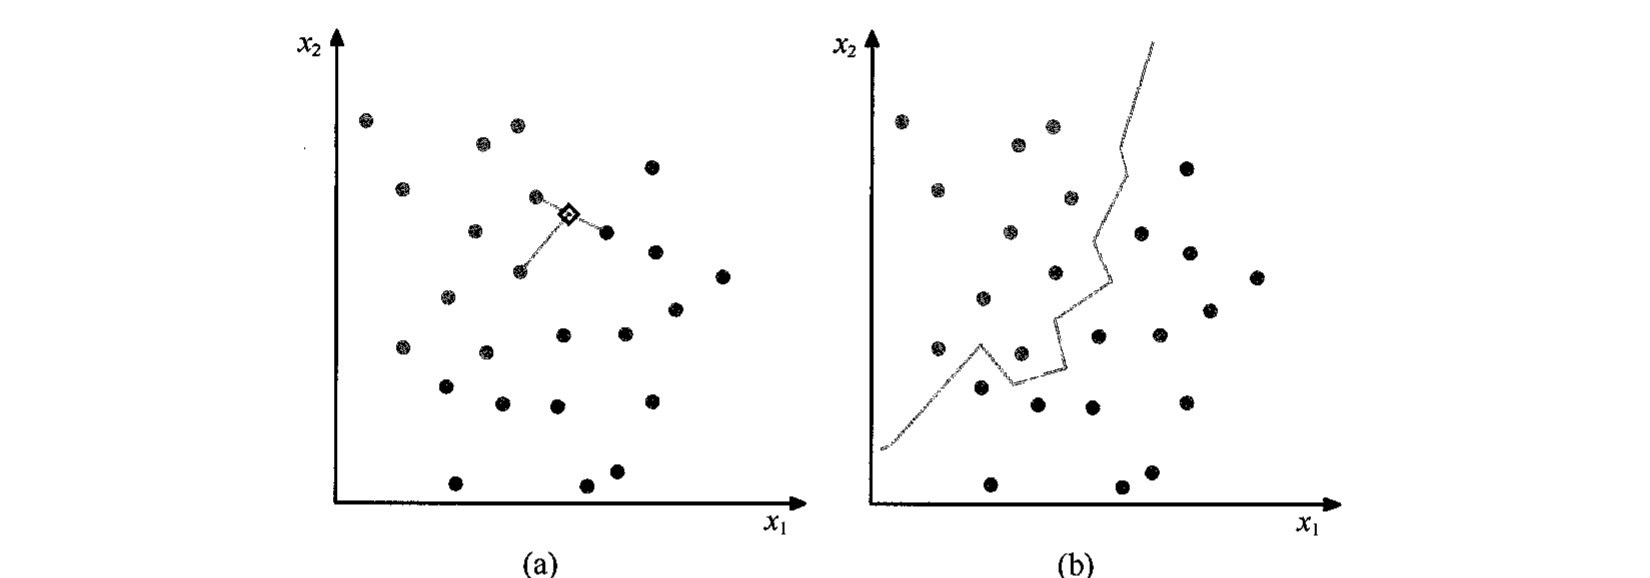
\includegraphics[width=0.92\textwidth]{ch03-fig3-16-knn-classify.png}
  \caption{(a)~在 $K$ 近邻分类器中，一个用黑色菱形表示的新点根据 $K$ 个最接近的训练数据点被归类为类别成员最多的那个类别，在本例中 $K=3$。(b)~在最近邻（$K=1$）分类器中，所得到的决策边界由超平面组成，每个超平面是由来自不同类别点对的垂直平分线构造的。}
  \label{figure:ch03-近邻分类}
\end{figure}

最近邻（$K=1$）分类器的一个有趣特性是，在 $N\to\infty$ 的情况下，错误率永远不会超过最优分类器（即使用真实类别分布的分类器）的最小可实现错误率的两倍（Cover and Hart, 1967）。

到目前为止，我们已经讨论了 $K$ 近邻方法和核密度估计，它们都需要存储整个训练集。如果数据集很大，计算成本将十分高昂。为了抵消这种影响，可以构建基于树的搜索结构，引入一些一次性的额外计算，以便高效地找到（近似的）近邻，而无须对整个数据集进行全量搜索。然而，这些非参数化方法的使用场景仍然受到严重制约。另外，我们已经看到简单的参数化模型仅能表示非常有限的分布形式。因此我们需要找到一些非常灵活的密度模型，它们的复杂度可以独立于训练集的大小而进行控制，深度神经网络可以实现这一点。

\begin{remark}（重构新增）
这一收尾段把全章的两条线索接了起来：参数化模型（如单个 Gauss 分布）表达力有限，非参数化模型（直方图、核密度、最近邻）表达力强却需要保存全部数据、计算随 $N$ 线性增长。深度神经网络提供了第三条路——用固定数量的参数表示高度灵活的分布，从而同时获得参数模型的效率与非参数模型的适应性。

“Cover-Hart 定理”给出的 $2$ 倍上界是最近邻方法最重要的理论保证，它说明哪怕最简单的 $K=1$ 规则在样本无限时也接近最优；但其前提是 $N\to\infty$ 且数据独立同分布，在有限样本、高维情形下这一保证并不提供实际性能的承诺。
\end{remark}

\end{document}
